\chapter{Estado del arte}

La estructura por capas de Android permite un sistema potente con una seguridad robusta. Cada aplicación se ejecuta en un entorno aislado (\textit{sandbox}) que incluye la propia aplicación, el \textit{framework} que utiliza y bibliotecas nativas del sistema; las comunicaciones entre las distintas aplicaciones están securizadas y cuenta con un amplio conjunto de permisos declarados por la aplicación y otorgados por el usuario. Cada capa es independiente de la anterior y supone que la que está inmediatamente por debajo ya está securizada (Figura~\ref{fig:stack}). Las diferentes partes del hardware que dan acceso a componentes arriesgados (\textit{TrustZone}) solo pueden ser utilizados por aplicaciones de confianza para que el SO permita el acceso.

Pero, a pesar de todo, como ya hemos podido comprobar, los dispositivos Android siguen sufriendo ataques, siguen siendo infectados y siguen teniendo vulnerabilidades.

\begin{figure}[H]
\centering
	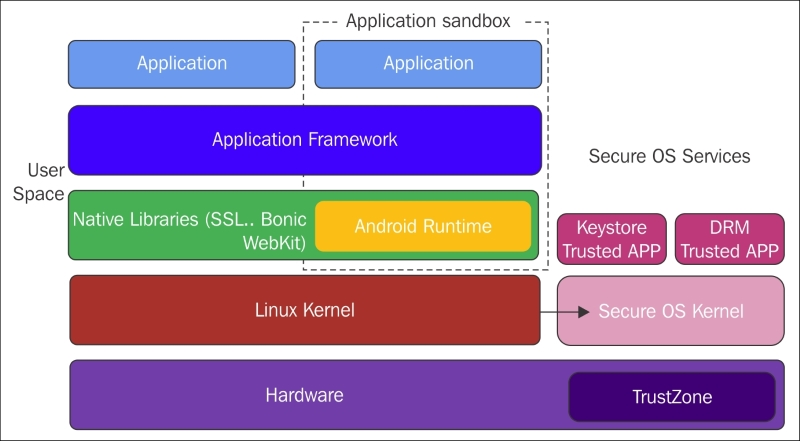
\includegraphics[scale=1.8]{img/android-stack.jpg}
	\caption{Modelo de seguridad de Android \textit{(Tahiri, 2016)}}
	\label{fig:stack}
\end{figure}

Hay muchas empresas que se encargan solo y exclusivamente de crear software capaz de detectar malware en todos los dispositivos, ya sean ordenadores, teléfonos, tabletas... en los distintos sistemas operativos disponibles para proteger activamente a los usuarios. Empresas como \textbf{McAfee}, \textbf{NowSecure}, \textbf{TeleSign} o el propio \textbf{Google} se encargan de crear detectores de malware y antivirus para móviles (entre otras tecnologías) que evitan, en la medida de lo posible, que nuestros dispositivos se vean afectados.

Los antivirus de hoy en día son capaces de detectar las amenazas de manera efectiva en la mayoría de los casos\hypersetup{citecolor=red}\cite{antimalware} mucho mejor de lo que lo hacían en el pasado. Han evolucionado para detener la actividad de cada vez más variantes de malware, pero no son capaces de neutralizarlos todos, pues el malware también evoluciona a pasos agigantados.

Debido a la enorme cantidad de malware existente y a todas las familias y subfamilias de cada uno con sus respectivas variantes, la detección y el análisis de malware es una tarea compleja que se divide en tres fases\hypersetup{citecolor=red}\cite{malwaredetection}:

\begin{enumerate}
	\item \textbf{Detección}: en esta fase se intenta localizar el malware que ha infectado el dispositivo.
	\item \textbf{Identificación}: tras la detección, se trata de identificar la familia del malware y, si es posible, la subfamilia y la variante. Identificar el malware no siempre es posible, pues podemos encontrarnos con una actividad anormal o extraña que nos dificulte el reconocimiento, o bien podemos encontrarnos con un malware nuevo que explota una vulnerabilidad del día cero y que no sabemos reconocer.
	\item \textbf{Eliminación}: tras haber identificado el malware, se procede a su eliminación para evitar que siga propagándose. Es importante destacar que no siempre es posible eliminarlo (ya sea porque no lo hemos podido detectar o porque no hemos podido identificarlo), y que por este motivo es importante mantener siempre copias de seguridad de todos los datos importantes.
\end{enumerate}

\section{Detección de malware}

Antes de entrar en formas específicas de detectar malware en un dispositivo Android, es necesario hablar de los tipos de análisis y técnicas existentes que pueden llevarse a cabo para después poder encajar este trabajo y algunos otros ejemplos en el marco de detección.

\subsection{Análisis de malware}

Vamos a centrarnos ahora en la identificación de malware según los diferentes tipos de análisis existentes\hypersetup{citecolor=red}\cite{analysis}. Son:

\begin{itemize}
	\item \textbf{Análisis estático}: esta técnica busca malware en la aplicación sin necesidad de ejecutarla usando un enfoque de análisis basado en firmas. Para ello, puede utilizar técnicas de ingeniería inversa para reconstruir el código fuente a partir del ejecutable y buscar comportamientos sospechosos o centrarse en los metadatos de la aplicación e intentar encontrar patrones que puedan indicar que la aplicación es maligna (llamadas sospechosas a distintas APIs, uso de bibliotecas externas sospechosas...). Hay formas de evitar que el malware sea descubierto mediante este tipo de análisis, como por ejemplo utilizar código ofuscado (que dificulta su lectura comprimiendo y cifrando el malware, añadiendo código muerto, sustituyendo instrucciones por otras equivalentes, etc).
	\item \textbf{Análisis dinámico}: supone la ejecución del malware en un entorno aislado y controlado (denominado \textit{sandbox environment}) que evita que el sistema anfitrión en el que se está analizando acabe infectado. Este tipo de análisis se enfoca en el comportamiento: trata de detectar acciones extrañas o sospechosas, y utiliza dichas acciones para la clasificación en programas benignos o malware. Se pueden utilizar diferentes tecnologías como depuradores de código para ver la ejecución paso a paso y comprobar los efectos del malware en el sistema, software de instrumentación para analizar las llamadas al sistema, herramientas software para detectar cambios en los registros y escrituras de memoria... Al igual que en el caso del análisis estático, hay métodos para evitar que la aplicación maligna sea descubierta: detectar si se está ejecutando en un entorno virtual o si el depurador está activo, dificultar, confundir o impedir los volcados de memoria...
	\item \textbf{Análisis híbrido}: fusiona las dos técnicas anteriores. Normalmente se analiza primero el código del ejecutable y después se ejecuta en un entorno aislado para monitorizar el comportamiento. Esta técnica recopila las ventajas de las dos anteriores para dar lugar a un análisis más efectivo, aunque es poco usado en teléfonos móviles.
\end{itemize}

\subsection{Técnicas de detección}

Según las técnicas utilizadas para la detección en Android, se pueden clasificar en tres\hypersetup{citecolor=red}\cite{detection}:

\begin{itemize}
	\item \textbf{Basada en firmas}: esta ténica se basa en comparar la firma de la aplicación o el patrón de actividad con otras firmas o patrones presentes en una base de datos que contiene ataques y malware ya conocido. La base de datos se actualiza constantemente, cada vez que se encuentra una nueva firma de una aplicación maligna, pero esta técnica no es válida en el caso de encontrarnos con malware del día cero o en el caso de que el código maligno se cargue de forma dinámica.\hypersetup{citecolor=red}\cite{firma} es un ejemplo de detector de malware que utiliza esta técnica.
	\item \textbf{Basada en anomalías}: está basada en heurísticas y es capaz de detectar malware del día cero, a diferencia de la técnica basada en firmas. Se trata de monitorizar la actividades que el dispositivo lleva a cabo con regularidad con el fin de detectar algún comportarmiento que se salga del patrón usual; cada comportamiento detectado es clasificado en \textit{normal} y \textit{anómalo}, como\hypersetup{citecolor=red}\cite{anomalias}. Esto significa que el sistema debe reconocer de antemano las actividades normales, lo que supone un entrenamiento y testeo previos.
	\item \textbf{Basada en especificaciones}: es un subtipo de detección basada en anomalías que tiene en cuenta el alto ratio de falsas alarmas producidas por la técnica anterior. En lugar de centrarse en los comportamientos en sí de cada aplicación, tiene en cuenta un conjunto extra de reglas que considera normales para determinar si la actividad que está llevando a cabo una aplicación que se ha salido de la ``normalidad'' es verdaderamente maliciosa o no, como\hypersetup{citecolor=red}\cite{espec}. Supone una capa añadida de comprobación a la técnica basada en anomalías, con la intención de reducir el número de falsos positivos.
\end{itemize}

\section{Detección y análisis de malware en Android}

La mayoría de técnicas de detección en Android utilizan un análisis estático\hypersetup{citecolor=red}\cite{martin}, que se centra en la información extraída del archivo \textit{AndroidManifest.xml}, las llamadas a funciones de la API de Android (examinando el código) o la información extraída del tráfico de red. Es más, muchas veces contienen un conjuto de expresiones regulares que especifican secuencias de instrucciones que pueden ser consideradas maliciosas, dando lugar por tanto a una técnica de detección basada en firmas. No obstante, como ya se ha explicado antes, esta forma de detectar malware se queda muy atrás en el momento en el que entra en juego un malware nuevo o malware con carga dinámica de código.

El análisis dinámico también es posible, pero mucho más restringido de lo que sería si el dispositivo fuera, por ejemplo, un ordenador. Las restricciones a las que nos enfrentamos en un teléfono dificultan el análisis dinámico que se ha conocido hasta ahora; para llevarlo es necesario instalar una aplicación que lleve a cabo dicho análisis, pero muchas veces este abordaje del problema provoca una caída del rendimiento del dispositivo y un gasto extra de batería. No obstante, hay ejemplos de análisis dinámico en Android, como aquellas aplicaciones que examinan las llamadas a las funcionas de la API de Android (estudiando el comportamiento, sin mirar el código), o aquellas que detectan la carga dinámica de código malicioso.

El análisis híbrido, aunque muy eficaz y común en análisis y detección de malware en ordenadores, no es el acercamiento que se utiliza en teléfonos móviles, pues requiere de tiempo, memoria extra y una capacidad de procesamiento que a veces los dispositivos no poseen.

En este trabajo se utiliza la infomación relativa a los permisos declarados en el archivo \textit{AndroidManifest.xml} antes mencionado; la recolección de los permisos de una aplicación para averiguar su clasificación entra en el análisis estático, puesto que se utilizan los metadatos de la aplicación sin necesidad de ejecutarla.

\section{Algunos trabajos sobre detección de malware}

El campo de la detección y análisis de malware en Android es un terreno al que aún le queda mucha exploración por delante. Se han hecho muchos estudios y se han desarrollado técnicas para la detección pero aún no se ha establecido ninguna de ellas como la mejor o la que arroja mejores resultados. Hay diversos artículos y numerosos trabajos donde se describen diferentes tipos de análisis utilizando distintas técnicas con el objetivo de encontrar un detector que ofrezca la mayor precisión.

Hablando del lugar en el que se lleva a cabo el análisis, puede hacerse dentro del propio dispositivo o fuera de éste. Algunos detectores realizan el análisis fuera del dispositivo, como por ejemplo\hypersetup{citecolor=red}\cite{cloud}, que debido a que lleva a cabo un análisis híbrido que requiere de mucha capacidad computacional, hace uso de la nube para la ejecución del análisis.

Ahora analicémos algunos trabajos de detección de malware para poder comparalos más tarde con \textit{Android Shield}.

\subsection{\textit{Detector de malware en Android usando características de grano fino}}

En\hypersetup{citecolor=red}\cite{jiang} utiliza un análisis estático, ya que, de forma análoga a \textit{Android Shield}, hace uso de un conjunto de permisos extraídos del \textit{AndroidManifest.xml} para clasificar si una aplicación es benigna o maliciosa. No obstante, a diferencia de \textit{Android Shield}, los permisos que utiliza son tanto peligrosos como no peligrosos.

Utiliza un método denominado \textit{fine-grained dangerous permission} (FDP) con el que amplian significativamente el número de permisos utilizados, clasificándolos según el uso que cada aplicación le dé. Es decir, FDP toma un permiso, como por ejemplo \textsc{WRITE\_SMS}, y lo desgrana en cuatro tipos: A (si lo utiliza como parte de la actividad de la app), B(si lo utiliza como parte de su actividad siendo una aplicación de difusión o \textit{broadcast}), D (si aparentemente no lo utiliza o si lo carga dinámicamente), I (si la aplicación invoca funciones sensibles de la API).

El estudio llevado a cabo con FDP en la detección de malware utiliza cuatro técnicas diferentes de Machine Learning con el fin de hacer una comparativa entre ellos y buscar los resultados óptimos:

\begin{itemize}
	\item \textit{J48}, un algoritmo basado en un árbol de decisiones. Es el algoritmo con mejores resultados en este estudio.
	\item \textit{K-Nearest Neighbor} o K-Vecinos más cercanos (KNN), un algoritmo que clasifica un objeto según los ejemplos que hay más cercanos a él.
	\item \textit{Naives Bayes} o Bayes ingenuo (NB), un algoritmo que clasifica un objeto sin tomar en cuenta la posible relación entre las características usadas en la clasificación.
	\item \textit{Support Vector Machine} o Máquina de Vector Soporte (SVM), un algortimo que busca la mayor separación entre los objetos de los dos subconjuntos de clasificación.
\end{itemize}

\subsection{\textit{Análisis de permisos para detección de malware en Android}}

En\hypersetup{citecolor=red}\cite{giang} también lleva a cabo un análisis estático de la aplicación. Al igual que el ejemplo anterior, utiliza un conjunto de permisos (aunque mucho más reducido) para detectar malware en Android. En este caso se usa un algoritmo basado en un árbol de decisiones, que clasifica si una aplicación es begnina o maliciosa según los permisos que declara del conjunto preestablecido como ``potencialmente proveniente de un malware''. El conjunto está compuesto por permisos tanto peligrosos como no peligrosos, un total de 13, aquellos utilizados más comúnmente en las aplicaciones, ya sean benignas o no.

Cada permiso utilizado tiene un peso asignado según el nivel de peligrosidad (es decir, según la información que dicho permiso puede arriesgar o la funcionalidad de la que va a hacer uso). El cálculo del valor de cada permiso a la hora de detectar si la aplicación es malware o no queda reflejado en la siguiente ecuación:

\[
P = \frac{S\cdot W}{S\cdot W+N}
\]

donde $S$ representa el número total de permisos peligrosos utilizados en el conjunto, $W$ es el peso asignado al permiso y $N$ es el número de permisos ``neutrales'' (no peligrosos) utilizados en el conjunto.

\subsection{\textit{Identificación de permisos significativos para detección de malware basado en Machine Learning en Android}}

En \hypersetup{citecolor=red}\cite{sigpid} se lleva a cabo un estudio previo para reducir el número de permisos utilizados (mediante la poda a varios niveles de la matriz original de permisos) y quedarse solo con los que son significativos a la hora de diferenciar entre aplicaciones benignas y malware. El número de permisos utilizados es solo 22, menos que los permisos que Google considera peligrosos; es más, la mayoría de los permisos del conjunto utilizado no son permisos peligrosos.

Una vez que el conjunto de permisos está establecido, utilizan dos algoritmos diferentes para quedarse con el que ofrece mejores resultados: el algoritmo SVM, con el que alcanzan una precisión del 91.22\% y el algoritmo FT (\textit{Functional Tree}), con el que alcanzan una precisión del 93.62\%.

\subsection{\textit{Detección de malware en Android basada en permisos}}

En \hypersetup{citecolor=red}\cite{aung} también se utiliza un análisis estático basado en el uso de permisos. De forma similar al resto de trabajos y a \textit{Android Shield}, hace una reducción del número de permisos utilizados para eliminar el ruido a la hora de entrenar el modelo. Para ello utiliza el método de ganancia de información (\textit{information gain}), un método que mide la entropía para seleccionar aquellas características que dan más información al modelo. La siguiente ecuación muestra la ganancia de la característica $A$ dentro de un conjunto de ejemplos dados en $S$

\[
Ganancia(S,A) = Entropia(S)-\sum_{V\in Valores(A)\cdot \mid S\mid} \mid SV\mid Entropia(SV)
\]

Una vez elegidos los permisos que se van a usar, utiliza el algoritmo K-medias (\textit{K-means clustering}), un algoritmo de agrupamiento en el que cada objeto (en este caso cada aplicación) pertenece al conjunto $K$ con el valor medio más cercano.

\subsection{\textit{Detección de malware en Android usando LSI}}

\hypersetup{citecolor=red}\cite{kumar} hace uso de tres características diferentes en su análisis estático: permisos, códigos de operación (\textit{Opcodes}) e \textit{intents}. 

Ya que el conjunto de características es muy amplio al principio, se utiliza una técnica denominada \textit{Latent Semantic Indexing} (Indexación semántica latente) o LSI, un método mediante el cual se reduce la dimensionalidad del problema gracias al uso de una técnica matemática llamada \textit{Singular Value Decomposition} o SVD. Es una técnica muy similar al PCA (ambos están estrechamente relacionados), aunque el SVD es mucho más utilizado en el procesamiento del lenguaje natural.

El SVD se combina con distintos algoritmos de \textit{Machine Learning} para deducir si una aplicación Android es maligna o benigna. Los algoritmos utilizados son:

\begin{itemize}
	\item \textit{Logic regression} o regresión logística, un algoritmo que clasifica una variable categórica (es decir, que solo puede adoptar un número limitado de categorías, en este caso aplicación benigna o maligna) según las características independientes.
	\item \textit{Random forest}, un algoritmo que crea varios árboles de decisiones diferentes durante el entrenamiento para después sacar el promedio de todos ellos. Es el algoritmo con mayor precisión en este trabajo.
	\item El algoritmo KNN, anteriormente explicado.
	\item Y el SVM, también explicado previamente.
\end{itemize}

\subsection{\textit{SFDroid: detección de malware en Android usando características estáticas}}

En \hypersetup{citecolor=red}\cite{garg} se analizan los componentes declarados en el \textit{AndroidManifest.xml} para llevar a cabo un análisis estático y determinar cuál de estos componentes es más efectivo para detectar malware. Se centran en seis componentes diferentes: permisos, \textit{intents}, componentes hardware, \textit{content providers}, \textit{broadcast receivers} y servicios de los que hacen uso y que están declarados en el \textit{AndroidManifest.xml}.

Puesto que son muchos componentes, primero se lleva a cabo una clasificación basada en la frecuencia de aparición de las características tanto en aplicaciones benignas como en malware. Con las frecuencias construyen dos clasificaciones diferentes: una con las características más utilizadas en malware y otra con las características más utilizadas en aplicaciones benignas. Tras esto, se calcula un umbral para eliminar aquellas características que tienen un ratio bajo de aparición.

Una vez que se tienen los conjuntos definitivos (separados por el tipo de componente), llevan a cabo los análisis utilizando tres algoritmos diferentes: \textit{Naives Bayes}, \textit{random forest} y SVM. Con los resultados dados por los algortimos se determina cuál de los seis componentes arroja mejores resultados a la hora de diferenciar entre aplicaciones benignas o maliciosas.

Utilizando solo uno de los componentes se pueden alcanzar tasas altas de acierto, pero ninguna tan alta como una combinación de las características más significativas de cada componente.

\subsection{\textit{Detección de malware en Android con permisos declarados en AndroidManifest.xml}}

En \hypersetup{citecolor=red}\cite{todd}, al igual que otros trabajos anteriores y que el propio \textit{Android Shield}, se utilizan solamente los permisos declarados en el \textit{AndroidManifest.xml} para hacer una clasificación que divida las aplicaciones en malignas o benignas.

Utilizando diferentes algoritmos de \textit{Machine Learning} como SVM, \textit{Naives Bayes}, \textit{K-means} y \textit{random forest}, se lleva a cabo un estudio con alrededor de 5000 muestras.

En este trabajo el algoritmo con mejores resultados es el \textit{random forest}, aunque la precisión que obtienen dista mucho de la obtenida en los demás trabajos.

\subsection{\textit{Maldozer: framework para detección de malware usando aprendizaje automático}}

En \hypersetup{citecolor=red}\cite{maldozer}, a diferencia de todos los trabajos anteriores, se lleva a cabo un análisis dinámico para detectar malware. En lugar de utilizar los permisos, en este caso se utilizan lan llamadas a la API de Android para detectar comportamientos extraños en las aplicaciones; se centra especialmente en las llamadas peligrosas, aquellas que hacen uso de componentes hardware o software que pueden ser arriesgados. Es capaz de detectar malware del día cero.

Para llevar a cabo el análisis utiliza una red neuronal y diferentes datasets con los que entrena y testea el modelo creado.

\subsection{\textit{RiskRanker: detección de malware del día cero en Android}}

En \hypersetup{citecolor=red}\cite{grace} también se lleva a cabo un análisis dinámico. No obstante, en este caso está orientado a detectar malware del día cero. Para ello se crea un detector escalable que analiza la carga dinámica de código en las aplicaciones. Después dicho código es analizado en busca de código maligno.

Aunque en este trabajo no se indica la precisión, sí se indica el número de aplicaciones maliciosas detectadas: 718 muestras provenientes de 29 familias diferentes. Entre las aplicaciones, 322 eran malware del día cero.

\section{Comparativa entre trabajos}

En la Tabla~\ref{tab:comp} vemos una comparativa de estos trabajos. En los trabajos que utilizan diferentes algotimos se muestra la precisión dada por cada uno.

\begin{table}[H]
\centering
\begin{tabular}{|c|c|c|c|}
\hline
\textbf{Trabajo}   & \textbf{Características utilizadas} & \textbf{Algoritmos utilizados} & \textbf{Precisión} \\ \hline
\multirow{4}{*}{\hypersetup{citecolor=red}\cite{jiang}} & \multirow{4}{*}{Permisos} & J48                & 94\%               \\ \cline{3-4} 
                   & & KNN                & 93.7\%             \\ \cline{3-4} 
                   & & NB                 & 92.9\%             \\ \cline{3-4} 
                   & & SVM                & 92\%               \\ \hline
\hypersetup{citecolor=red}\cite{giang}                  & Permisos & Decision tree      & 85\%               \\ \hline
\multirow{2}{*}{\hypersetup{citecolor=red}\cite{sigpid}} & \multirow{2}{*}{Permisos} & SVM                & 91.22\%            \\ \cline{3-4} 
                   & & FT                 & 93.62\%            \\ \hline
\hypersetup{citecolor=red}\cite{aung}                  & Permisos & K-means clustering           & 91.8\%             \\ \hline
\multirow{4}{*}{\hypersetup{citecolor=red}\cite{kumar}} & \multirow{4}{*}{Permisos, \textit{Opcodes} e \textit{intents}} & Logic regression                & 92.21\%               \\ \cline{3-4} 
                   & & Random forest                & 93.92\%             \\ \cline{3-4} 
                   & & KNN                 & 91.24\%             \\ \cline{3-4} 
                   & & SVM                & 91.97\%               \\ \hline
\multirow{3}{*}{\hypersetup{citecolor=red}\cite{garg}} & \multirow{3}{*}{\shortstack{Permisos, \textit{intents}, componentes hardware, \\ \textit{content providers}, \textit{broadcast receivers} y\\ servicios}} & NB                & 90.78\%               \\ \cline{3-4} 
                   & & Random forest                & 94.89\%             \\ \cline{3-4} 
                   & & SVM                & 95.90\%               \\ \hline
\multirow{4}{*}{\hypersetup{citecolor=red}\cite{todd}} & \multirow{4}{*}{Permisos} & Random forest                & 81.53\%               \\ \cline{3-4} 
                   & & SVM                & 79.87\%             \\ \cline{3-4} 
                   & & Gaussian NB                 & 60.28\%             \\ \cline{3-4} 
                   & & K-means                & 80.54\%               \\ \hline
\hypersetup{citecolor=red}\cite{maldozer}                  & Llamadas a la API & Neural network           & 98.95\%             \\ \hline
\end{tabular}
\caption{Comparativa de trabajos}
\label{tab:comp}
\end{table}